\documentclass[conf]{new-aiaa}

\usepackage{amsmath,amssymb}
\usepackage{array}
\usepackage{float}
\usepackage{graphicx}
\usepackage{geometry}

\usepackage{booktabs}
\usepackage{diagbox}
\usepackage[table,xcdraw]{xcolor}

\usepackage{siunitx}
\usepackage{longtable,tabularx}
\usepackage{caption}
\usepackage{subcaption}

\usepackage{minted}
\usemintedstyle{autumn}
\setminted{linenos,breaklines,tabsize=4,xleftmargin=1.5em}

\title{VE401 Term Project 2\\
Rules of metrological testing for net quantity of products in prepackage with fixed content}
\author{Group 21\\
Yihao Liu (515370910207)
\footnote{Authors' names are in alphabet order.}
}
\affil{University OF Michigan - Shanghai Jiao Tong University Joint Institute, Shanghai, China}

\begin{document}

\maketitle

\begin{abstract}
    
\end{abstract}

\vspace{11cm}
\noindent Keywords: 

\newpage

\tableofcontents
\newpage


\section{Nomenclature}

{\renewcommand\arraystretch{1.0}
\noindent\begin{longtable*}{@{}l @{\quad=\quad} l@{}}
$N$ & total number of inspection lot
\end{longtable*}}

\newpage

\section{Problem Statement}

\subsection{Introduction}

Fatal force and fatal shooting by police are topics that attract headlines and trigger heated debate around the world. When we are discussing these topics, it’s important to have a clear image of what ``fatal police shooting'' is. Then we will discuss the pattern of police shootings regarding to the probability. 

According to the statistics from the Washington Post [3] 962 people have been shot and killed by police in the US in 2016, and 994 people were fatally shot by police in 2015. The Washington Post is compiling such a database of every fatal shooting in the United States by a police officer in the line of duty since Jan. 1, 2015. This database is based on news reports, public records, social media and other sources.

For the term ``fatal police shooting,'' the Post characterizes it as those shootings in which a police officer, in the line of duty, shoots and kills a civilian — the circumstances that most closely parallel the 2014 killing of Michael Brown in Ferguson, Mo., which began the protest movement culminating in Black Lives Matter and attracted attention to police accountability nationwide [4]. What is worth attention is that the Post is not tracking deaths of people ``in police custody, fatal shootings by off-duty officers or non-shooting deaths.''

\begin{figure}[H]
	\centering
	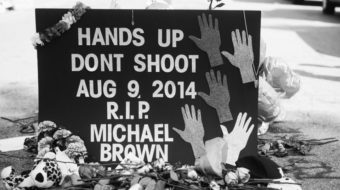
\includegraphics[width=0.7\linewidth]{intro.png}  
	\caption{Silent protest for police shooting of Michael Brown.}  
\end{figure}

Of course every single murder is a tragedy for those whom it affects, but for the bettering of the police service and the benefit of broader society we may wish to consider whether these ``shocking'' numbers lead to some patterns. In the following content, we carry out a statistical analysis on the mass shootings in the US from 2015 - 2018, exploring the distribution pattern, the dependence on weekday and month, then anticipating the number of police shootings in 2019.

\subsection{Overview}

First, we use \emph{Mathematica} to visualize the fatal police shooting from the data provided by \emph{WashingtonPost}\cite{} between January 1$^{\rm st}$,2015 and December 31$^{\rm st}$, 2018. The plot was shown in Figure \ref{fig:q2}.

\begin{figure}[!htbp]
	\centering
	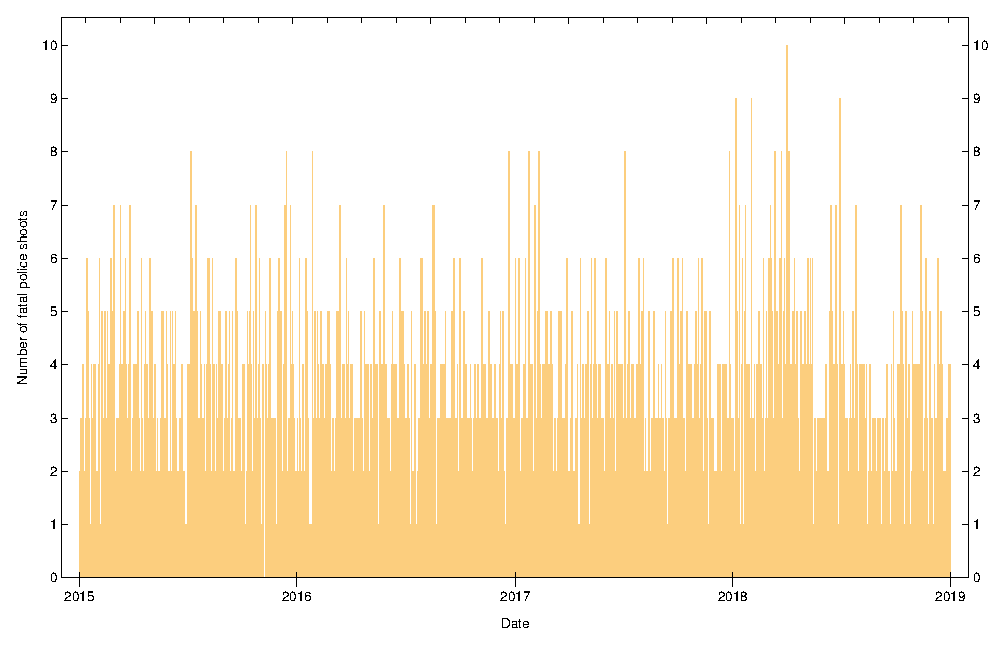
\includegraphics[width=0.9\linewidth]{q2/q2.eps}
	\caption{Number of fatal police shoots each day between January 1$^{\rm st}$,2015 and December 31$^{\rm st}$, 2018.}
	\label{fig:q2}
\end{figure}

Note that 2016 is a leap year, which means that there is one more day (February 29$^{\rm th}$) in 2016 than in the other three years, so the distance between 2016 and 2017 on the x-axis is slightly different from the distance between other years.

\subsection{Background}

In this project, we 

\subsubsection{Poisson distribution}
\label{title:poisson}

\newpage

\section{Description of work}

\subsection{Distribution of fatal police shootings between 2015 and 2018}

In the work of Spiegelhalter and Barnett\cite{}, the London homicides follow a Poisson distribution with parameter $k = 0.44$. We suggested that the distribution of fatal police shooting in the USA may be similar to that of London homicides, then we assumed that the police shootings follow a Poisson distribution with an unknown parameter $k$ and performed a goodness-of-fit test for Poisson distribution.

\subsubsection{Hypothesis test of data in four years between 2015 and 2018}\label{title:q3-1}

First, we collected the fatal police shootings between 2015 and 2018 altogether and performed a hypothesis test. There are 1461 days in these four years, so that the random sample size is $n=1461$. We used \emph{Mathematica} to categorize and analyze the data according to the number of fatal police shootings $X$ and corresponding observed frequency $O_i$, as shown in Table \ref{tab:q3-all-obs} and Figure \ref{fig:q3-all-obs}. \medskip

\begin{table}[!htbp]
\centering
\begin{tabular}{m{3cm}<{\centering}m{3cm}<{\centering}}
\toprule 
\toprule
Number of fatal police shootings $X$    & Observed Frequency $O_i$ \\
\noalign{\smallskip}\hline\noalign{\smallskip}
0  &   108    \\
1  &   287   \\
2  &   324    \\
3  &   310    \\
4  &   227    \\
5  &   116    \\
6  &   53    \\
7  &   21    \\
8  &   11    \\
9  &   3    \\
10  &  1     \\
\bottomrule 
\bottomrule\smallskip
\end{tabular}
\caption{Observed Frequency $O_i$ versus each number of fatal police shootings data between 2015 and 2018.}
\label{tab:q3-all-obs}
\end{table}

\begin{figure}[!htbp]
\centering
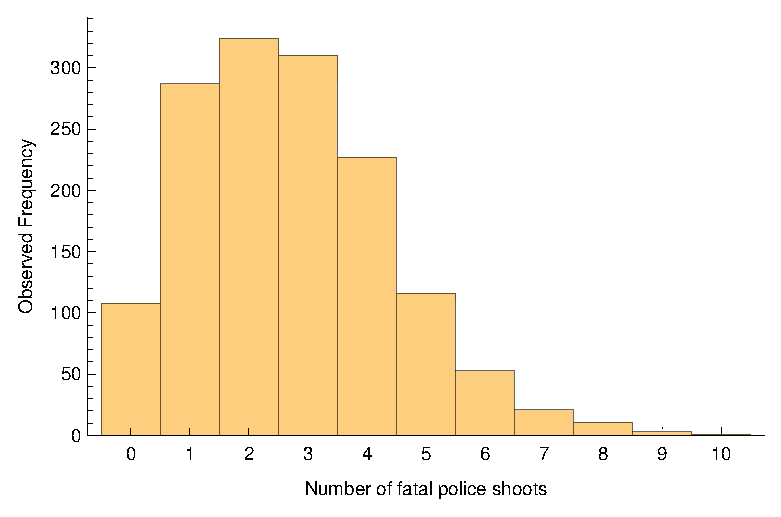
\includegraphics[height=7cm]{q3/q3-all-obs.eps}
\caption{Observed Frequency $O_i$ versus each number of fatal police shootings data between 2015 and 2018.}
\label{fig:q3-all-obs}
\end{figure}

The parameter $k$ of the assumed Poisson distribution is unknown and must be estimated from the data. According to \ref{title:poisson}, we know that a maximum-likelihood estimator for $k$ is the sample mean,
$$\hat{k} = \frac{1}{n}\sum_{i=1}^{10} X_iO_i = \frac{3943}{1461} \approx 2.69884.$$
We test 
$$H_0:{\rm the\ number\ of\ fatal\ police\ shootings\ follows\ a\ Poisson\ distribution\ with\ parameter\ }k = 2.69884.$$

In order to transform the test of Poisson distribution into a test of categorical distribution, we first calculate the estimated probability for each category,
$$P[X=i]=\frac{e^{-\hat{k}}\hat{k}^i}{i!},\quad{\rm for\ }i\in[0,9],i\in Z,$$
and typically
$$P[X=10]=1-\sum_{i=0}^9P[X=i]=1-\sum_{i=0}^9\frac{e^{-\hat{k}}\hat{k}^i}{i!}$$
for the last category. The expected frequency can be calculated by
$$E_i=nP[X=i].$$
The calculated results were shown in Table \ref{tab:q3-all-exp}. \medskip

\begin{table}[!htbp]
\centering
\begin{tabular}{m{3cm}<{\centering}m{3cm}<{\centering}m{3cm}<{\centering}m{3cm}<{\centering}}
\toprule 
\toprule
Number of fatal police shootings $X$ (Category $i$)
 & Observed Frequency $O_i$ 
& Expected Probability $P[X=i]$ & Expected Frequency $E_i$ \\
\noalign{\smallskip}\hline\noalign{\smallskip}
0  &   108   & 0.0672838  & 98.3016\\
1  &   287   & 0.181588   & 265.3\\
2  &   324   & 0.245038   & 358.0\\
3  &   310   & 0.220439   & 322.062\\
4  &   227   & 0.148732   & 217.298\\
5  &   116   & 0.0802808  & 117.29\\
6  &   53    & 0.0361108  & 52.7579\\
7  &   21    & 0.0139224  & 20.3407\\
8  &   11    & 0.0046968  & 6.86203\\
9  &   3     & 0.00140843 & 2.05772\\
$\geqslant$10 &   1     & 0.000499723& 0.730095\\
\bottomrule 
\bottomrule  \smallskip
\end{tabular}
\caption{Expected probability and frequency for the categorized fatal police shootings data between 2015 and 2018.}
\label{tab:q3-all-exp}
\end{table}

According to the Pearson Statistic, two generally stated criteria of  categorical distribution are
\begin{align*}
E_i=nP[X=i]\geqslant1 & \qquad {\rm for\ all\ }i=1,\dots,N,\\
E_i=nP[X=i]\geqslant5 & \qquad {\rm for\ 80\%\ of\ all\ }i=1,\dots,N,
\end{align*}
where $N$ is the number of the categories. In our data, we can find that $E_{10}=0.730095<1$, which doesn't satisfy the criteria. The problem can be solved by combining the last two categories, which makes
\begin{align*}
&O_9'=O_9+O_{10}=4,\\
&P[X\geqslant9]=P[X=9]+P[X\geqslant10]\approx 0.00190816,\\
&E_9'=nP[X\geqslant9]\approx2.78782.
\end{align*}
Now only one category has an expectation less than 5, and all of the categories have expectations greater then 1, which satisfies the criteria. The origin test is then equivalent to the test
$$H_0:{\rm the\ number\ of\ fatal\ police\ shootings\ follows\ a\ categorical\ distribution\ with\ parameters\ }E_i.$$

For $N = 10$ categories, the statistic
$$X^2=\sum_{i=0}^{N-1}\frac{(O_i-E_i)^2}{E_i}$$
then follows a chi-squared distribution with $N-1-m=10-1-1=8$
degree of freedom, where $m$ is the number of estimated parameters. With the data, we have
$$X^2\approx9.9049,$$
and we can reject $H_0$ at $\alpha$ level of significance if $X^2>\chi^2_{\alpha,8}$. When $\alpha\approx0.448876$,
$$\chi^2_{\alpha,8}\approx9.9049=X^2,$$
so the P-value of the test is $0.448876$, which is much larger than 0.05. \medskip

We also plotted Figure \ref{fig:q3-all-exp} to show the observed frequency $O_i$, expected Frequency $E_i$ and estimated Poisson distribution. The data fit the curve fine, which also gives evidence that it follow a Poisson distribution. \medskip

\begin{figure}[!htbp]
\centering
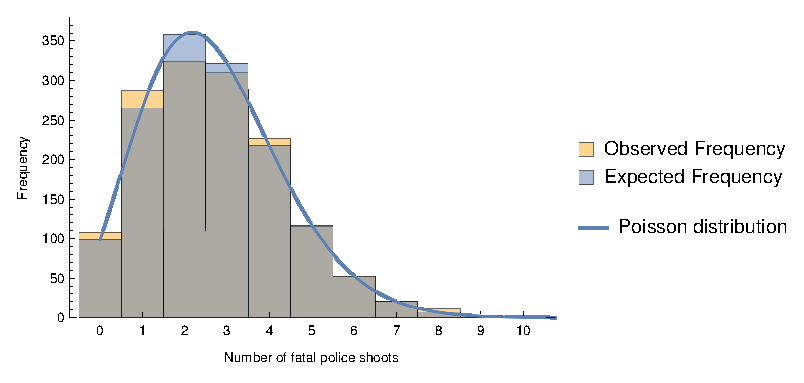
\includegraphics[height=7cm]{q3/q3-all-exp.eps}
\caption{Observed Frequency $O_i$, Expected Frequency $E_i$ and estimated Poisson distribution versus each number of fatal police shootings data between 2015 and 2018.}
\label{fig:q3-all-exp}
\end{figure}

In conclusion, we have no evidence to reject $H_0$, which means the fatal police shootings between 2015 and 2018 is likely to follow a Poisson distribution with $k=2.69884.$

\subsubsection{Hypothesis test of data in individual years}

The procedure of the hypothesis test of Poisson distribution in the individual years is exactly the same as that for all years (\ref{title:q3-1}), we will omit some detailed deduction and provide the results for each year individually.

\paragraph{Year 2015}\ 

The categorized data, expected probability and frequency were shown in Table \ref{tab:q3-2015-exp}. \medskip

\begin{table}[!htbp]
\centering
\begin{tabular}{m{3cm}<{\centering}m{3cm}<{\centering}m{3cm}<{\centering}m{3cm}<{\centering}}
\toprule 
\toprule
Number of fatal police shootings $X$ (Category $i$)
 & Observed Frequency $O_i$ 
& Expected Probability $P[X=i]$ & Expected Frequency $E_i$ \\
\noalign{\smallskip}\hline\noalign{\smallskip}
0  &   24   & 0.0654789  & 23.8998\\
1  &   73   & 0.178497   & 65.1515\\
2  &   87   & 0.243294   & 88.8024\\
3  &   69   & 0.221076   & 80.6926\\
4  &   55   & 0.150665   & 54.9925\\
5  &   33   & 0.0821431  & 29.9822\\
6  &   14   & 0.0373207  & 13.6221\\
7  &   8    & 0.0145339  & 5.30488\\
$\geqslant$8  &   2    & 0.0069918  & 2.55201\\
\bottomrule 
\bottomrule  \smallskip
\end{tabular}
\caption{Expected probability and frequency for the categorized fatal police shootings data in 2015.}
\label{tab:q3-2015-exp}
\end{table}

Here we have
\begin{align*}
&n=365,\\
&\hat{k} = \frac{1}{n}\sum_{i=1}^{10} X_iO_i = \frac{199}{73} \approx 2.72603,\\
&O_7'=O_7+O_8=10,\\
&P[X\geqslant7]=P[X=7]+P[X\geqslant8]\approx 0.0215257,\\
&E_9'=nP[X\geqslant9]\approx7.85688,\\
&X^2=\sum_{i=0}^{N-1}\frac{(O_i-E_i)^2}{E_i}=3.57557,\\
&P\approx0.893246.
\end{align*}

The P-value of the test is is much larger than 0.05, and the data fit the curve fine in Figure \ref{fig:q3-2015-exp}. We can claim that the fatal police shootings in 2015 and is likely to follow a Poisson distribution with $k=2.72603.$

\begin{figure}[!htbp]
\centering
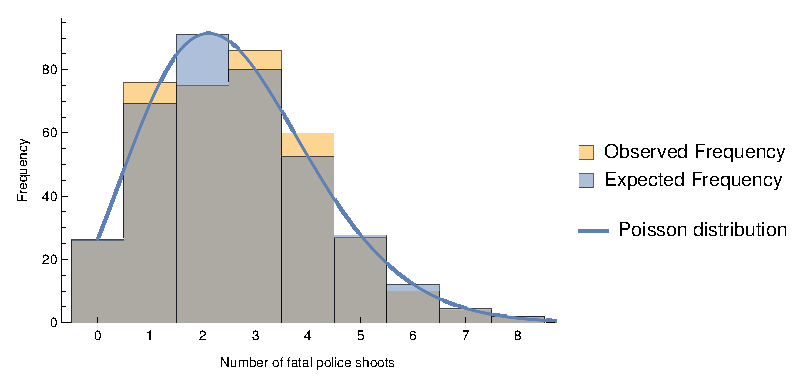
\includegraphics[height=7cm]{q3/q3-2015-exp.eps}
\caption{Observed Frequency $O_i$, Expected Frequency $E_i$ and estimated Poisson distribution versus each number of fatal police shootings data in 2015.}
\label{fig:q3-2015-exp}
\end{figure}

\paragraph{Year 2016}\ 

\begin{figure}[!htbp]
\centering
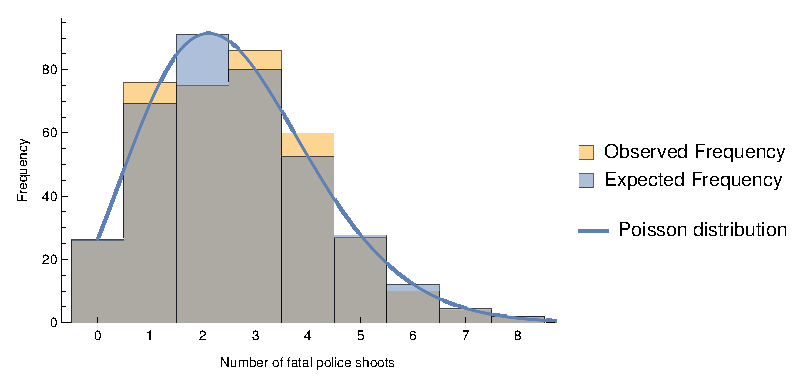
\includegraphics[height=7cm]{q3/q3-2016-exp.eps}
\caption{Observed Frequency $O_i$, Expected Frequency $E_i$ and estimated Poisson distribution versus each number of fatal police shootings data in 2016.}
\label{fig:q3-2016-exp}
\end{figure}

\paragraph{Year 2017}\ 

\begin{figure}[!htbp]
\centering
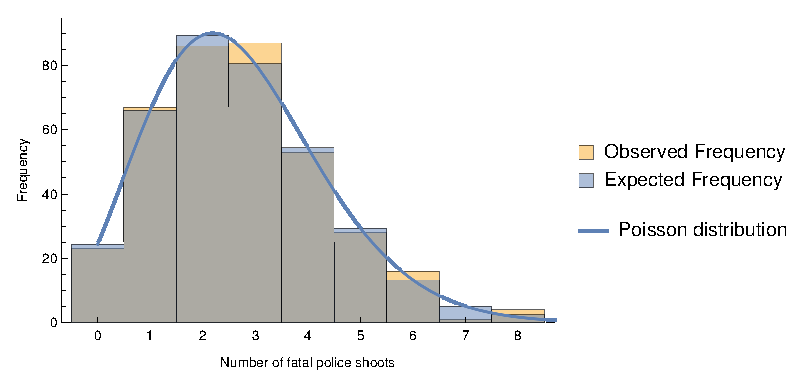
\includegraphics[height=7cm]{q3/q3-2017-exp.eps}
\caption{Observed Frequency $O_i$, Expected Frequency $E_i$ and estimated Poisson distribution versus each number of fatal police shootings data in 2017.}
\label{fig:q3-2017-exp}
\end{figure}

\paragraph{Year 2018}\ 

\begin{figure}[!htbp]
\centering
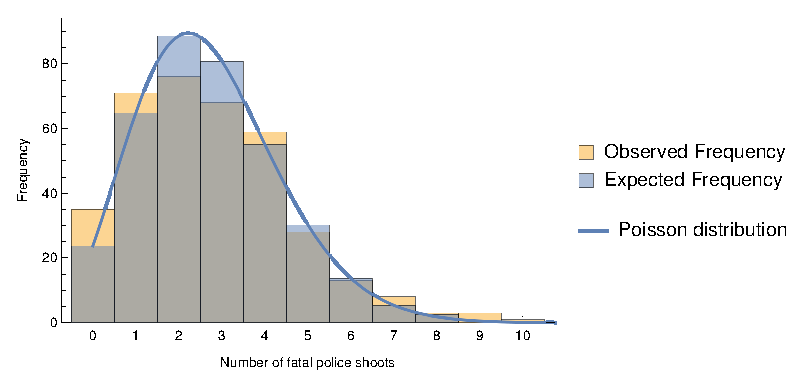
\includegraphics[height=7cm]{q3/q3-2018-exp.eps}
\caption{Observed Frequency $O_i$, Expected Frequency $E_i$ and estimated Poisson distribution versus each number of fatal police shootings data in 2018.}
\label{fig:q3-2018-exp}
\end{figure}

\subsection{Independence test of fatal police shootings}


\subsection{Confidence intervals of the distribution}

Let the ramdom variable $X$ denote the everyday occurrence of police shooting in the United States. We have verified that $X$ follows a Poisson distribution, $p(x)=\frac{(k)^{x}}{x !} e^{k}$. Now we are of interest in the confidence inverval for the parameter $k$. 

We have already known that the a maximum-likelihood estimator for $k$ is the sample mean, $\overline{X}$. 

Since our sample size is sufficient large, with the central limit theorem, it is advisable to say that our sample mean follows a normal distribution. Furthermore, we have a standard normal distribution
\begin{equation}
    Z=\frac{\overline{X}-k}{\sigma / \sqrt{n}} 
\end{equation}


We then need to find and estimator for the variance $\sigma^2$. With the property Poisson distribution. The variance of $X$ should be $Var X = k$. Therefore, the estimator for variance is the estimator for k, which is the sample mean, $\overline{X}$.

Now we rewrite the equ.1 as 
$$
Z = \frac{\hat{k}-k}{ \hat{k}/ \sqrt{n}}
$$
where $\hat{k}$ is the estimator for $k$, which is $\overline{X}$.

It is obvious that the a $(1 - \alpha)100\%$ confidence inverval is 
$$
\hat{k} \pm z_{\alpha / 2} \sqrt{\hat{k} / n}
$$

We can find that there were 3943 police shootings of the year 2015 to 2018. We can calclulate the mean occurrence of one day by
$$
\overline{X} = \frac{3943}{365+366+365+365} = 2.70 
$$
The 95\% confidence inverval can be calclulated as 
$$
2.70 \pm 1.96 \sqrt{2.7/3943} = (2.65 , 2.75)
$$


\subsection{Distribution of fatal police shootings in early 2019}

Suppose that the number of fatal police shoot between January and March 2019 follows a Poisson distribution with unknown parameter $k$. We want
to determine if there is evidence that this claim is false.

According to the data obtained from xxx, there are 90 days in this three months, so that the random sample size is $N=90$.

\begin{tabular}{cc}
Number & Frequency \\\hline
0 & 8 \\
1 & 16 \\
2 & 22 \\
3 & 18 \\
4 & 11 \\
5 & 7 \\
6 & 5 \\
7 & 2 \\
8 & 0 \\
9 & 1 
\end{tabular}

(according to some proofs in q2 copied from example 2.2.7)

We know that a maximum-likelihood estimator for $k$ is the sample mean,
$$\hat{k}=\overline{X}=\frac{1}{90}
(0\cdot8+1\cdot16+2\cdot22+3\cdot18+4\cdot11
+5\cdot7+6\cdot5+7\cdot2+9\cdot1)=\frac{41}{15}.$$

In order to apply the multinomial distribution, we first calculate
\begin{align*}
P[X=0]&=\frac{e^{-\hat{k}}\hat{k}^0}{0!}=0.0650023\\
P[X=1]&=\frac{e^{-\hat{k}}\hat{k}^1}{1!}=0.177673\\
P[X=2]&=\frac{e^{-\hat{k}}\hat{k}^2}{2!}=0.24282\\
P[X=3]&=\frac{e^{-\hat{k}}\hat{k}^3}{3!}=0.221236\\
P[X=4]&=\frac{e^{-\hat{k}}\hat{k}^4}{4!}=0.151178\\
P[X=5]&=\frac{e^{-\hat{k}}\hat{k}^5}{5!}=0.0826438\\
P[X=6]&=\frac{e^{-\hat{k}}\hat{k}^6}{6!}=0.0376488\\
P[X\geqslant7]&=1-\sum_{i=0}^6P[X=i]=0.0217996
\end{align*}

expected frequencies:
5.8502, 15.9906, 21.8538, 19.9112, 13.606, 7.43794, 3.38839, 1.96196

Last two added and get 5.35036.

$$X^2=\sum_{i=1}^N\frac{(O_i-E_i)^2}{E_i}=2.81152$$
$$N-1-m=7-1-1=5$$
$$\chi^2_{0.72,5}=2.81$$

So the P-value of the test is 0.72, too large, unable to reject Poisson distribution

$$\hat{k}_{2019}=\frac{41}{15}$$

\subsection{Prediction of fatal police shootings in 2019}

\section{References}

\subsection{Code}

\subsection{Bibliography}

\begin{thebibliography}{9}
\bibitem{horst}Horst Hohberger, \emph{VE401,Probabilistic Methods in Eng. Slides}, University OF Michigan - Shanghai Jiao Tong University Joint Institute, Shanghai, China

\end{thebibliography}

\end{document}
